\begin{figure*}
\raggedright
\begin{framed}
\begin{center}{\LARGE {\bf Model Card - Toxicity in Text}}\end{center} 
    \begin{minipage}{.45\textwidth}


{\bf Model Details} 
\begin{itemize}[leftmargin=*]
\item The TOXICITY classifier provided by Perspective API \cite{perspective_api}, trained to predict the likelihood that a comment will be perceived as toxic. 
\item Convolutional Neural Network.
\item Developed by Jigsaw in 2017.
\end{itemize}

{\bf Intended Use}
\begin{itemize}[leftmargin=*]
\item Intended to be used for a wide range of use cases such as supporting human moderation and providing feedback to comment authors.
\item Not intended for fully automated moderation.
\item Not intended to make judgments about specific individuals.
\end{itemize}

{\bf Factors}
\begin{itemize}[leftmargin=*]
\item Identity terms referencing frequently attacked groups, focusing on sexual orientation, gender identity, and race.
\end{itemize}

{\bf Metrics}
\begin{itemize}[leftmargin=*]
\item Pinned AUC, as presented in \cite{DixonEtAl2018}, which measures threshold-agnostic separability of toxic and non-toxic comments for each group, within the context of a background distribution of other groups.
\end{itemize}

{\bf Ethical Considerations}
\begin{itemize}[leftmargin=*]
\item Following \cite{conversation_ai}, the Perspective API uses a set of values to guide their work. These values are Community, Transparency, Inclusivity, Privacy, and Topic-neutrality. Because of privacy considerations, the model does not take into account user history when making judgments about toxicity.
\end{itemize}
%\vspace{5em}
%\begin{itemize}[leftmargin=*]
%\item Please see Figure \ref{fig:toxicity_analysis}.
%\end{itemize}
%\end{framed}
\vspace{1em}
 \end{minipage}
 \hspace{2em}
     \begin{minipage}{.45\textwidth}
%\caption{Example Model Card for a Toxicity Classifier}\label{fig:toxicity_card}
%\end{figure}
%\begin{figure}
%\begin{framed}
\vspace{2em}
{\bf Training Data} 
\begin{itemize}[leftmargin=*]
\item Proprietary from Perspective API.  Following details in \cite{DixonEtAl2018} and \cite{perspective_api}, this includes comments from a online forums such as Wikipedia and New York Times, with crowdsourced labels of whether the comment is ``toxic''.
\item ``Toxic'' is defined as ``a rude, disrespectful, or unreasonable comment that is likely to make you leave a discussion.''
\end{itemize}

{\bf Evaluation Data} 
\begin{itemize}[leftmargin=*]
\item A synthetic test set generated using a template-based approach, as suggested in \cite{DixonEtAl2018}, where identity terms are swapped into a variety of template sentences.
\item Synthetic data is valuable here because \cite{DixonEtAl2018} shows that real data often has disproportionate amounts of toxicity directed at specific groups. Synthetic data ensures that we evaluate on data that represents both toxic and non-toxic statements referencing a variety of groups. 
\end{itemize}

{\bf Caveats and Recommendations}
\begin{itemize}[leftmargin=*]
\item Synthetic test data covers only a small set of very specific comments. While these are designed to be representative of common use cases and concerns, it is not comprehensive.
\end{itemize}
\vspace{11em}
\end{minipage}
%\vspace{-2em}
{\bf Quantitative Analyses} \\
\hspace{-.65em}\begin{subfigure}{\textwidth}
%\vspace{1em}
\centering
%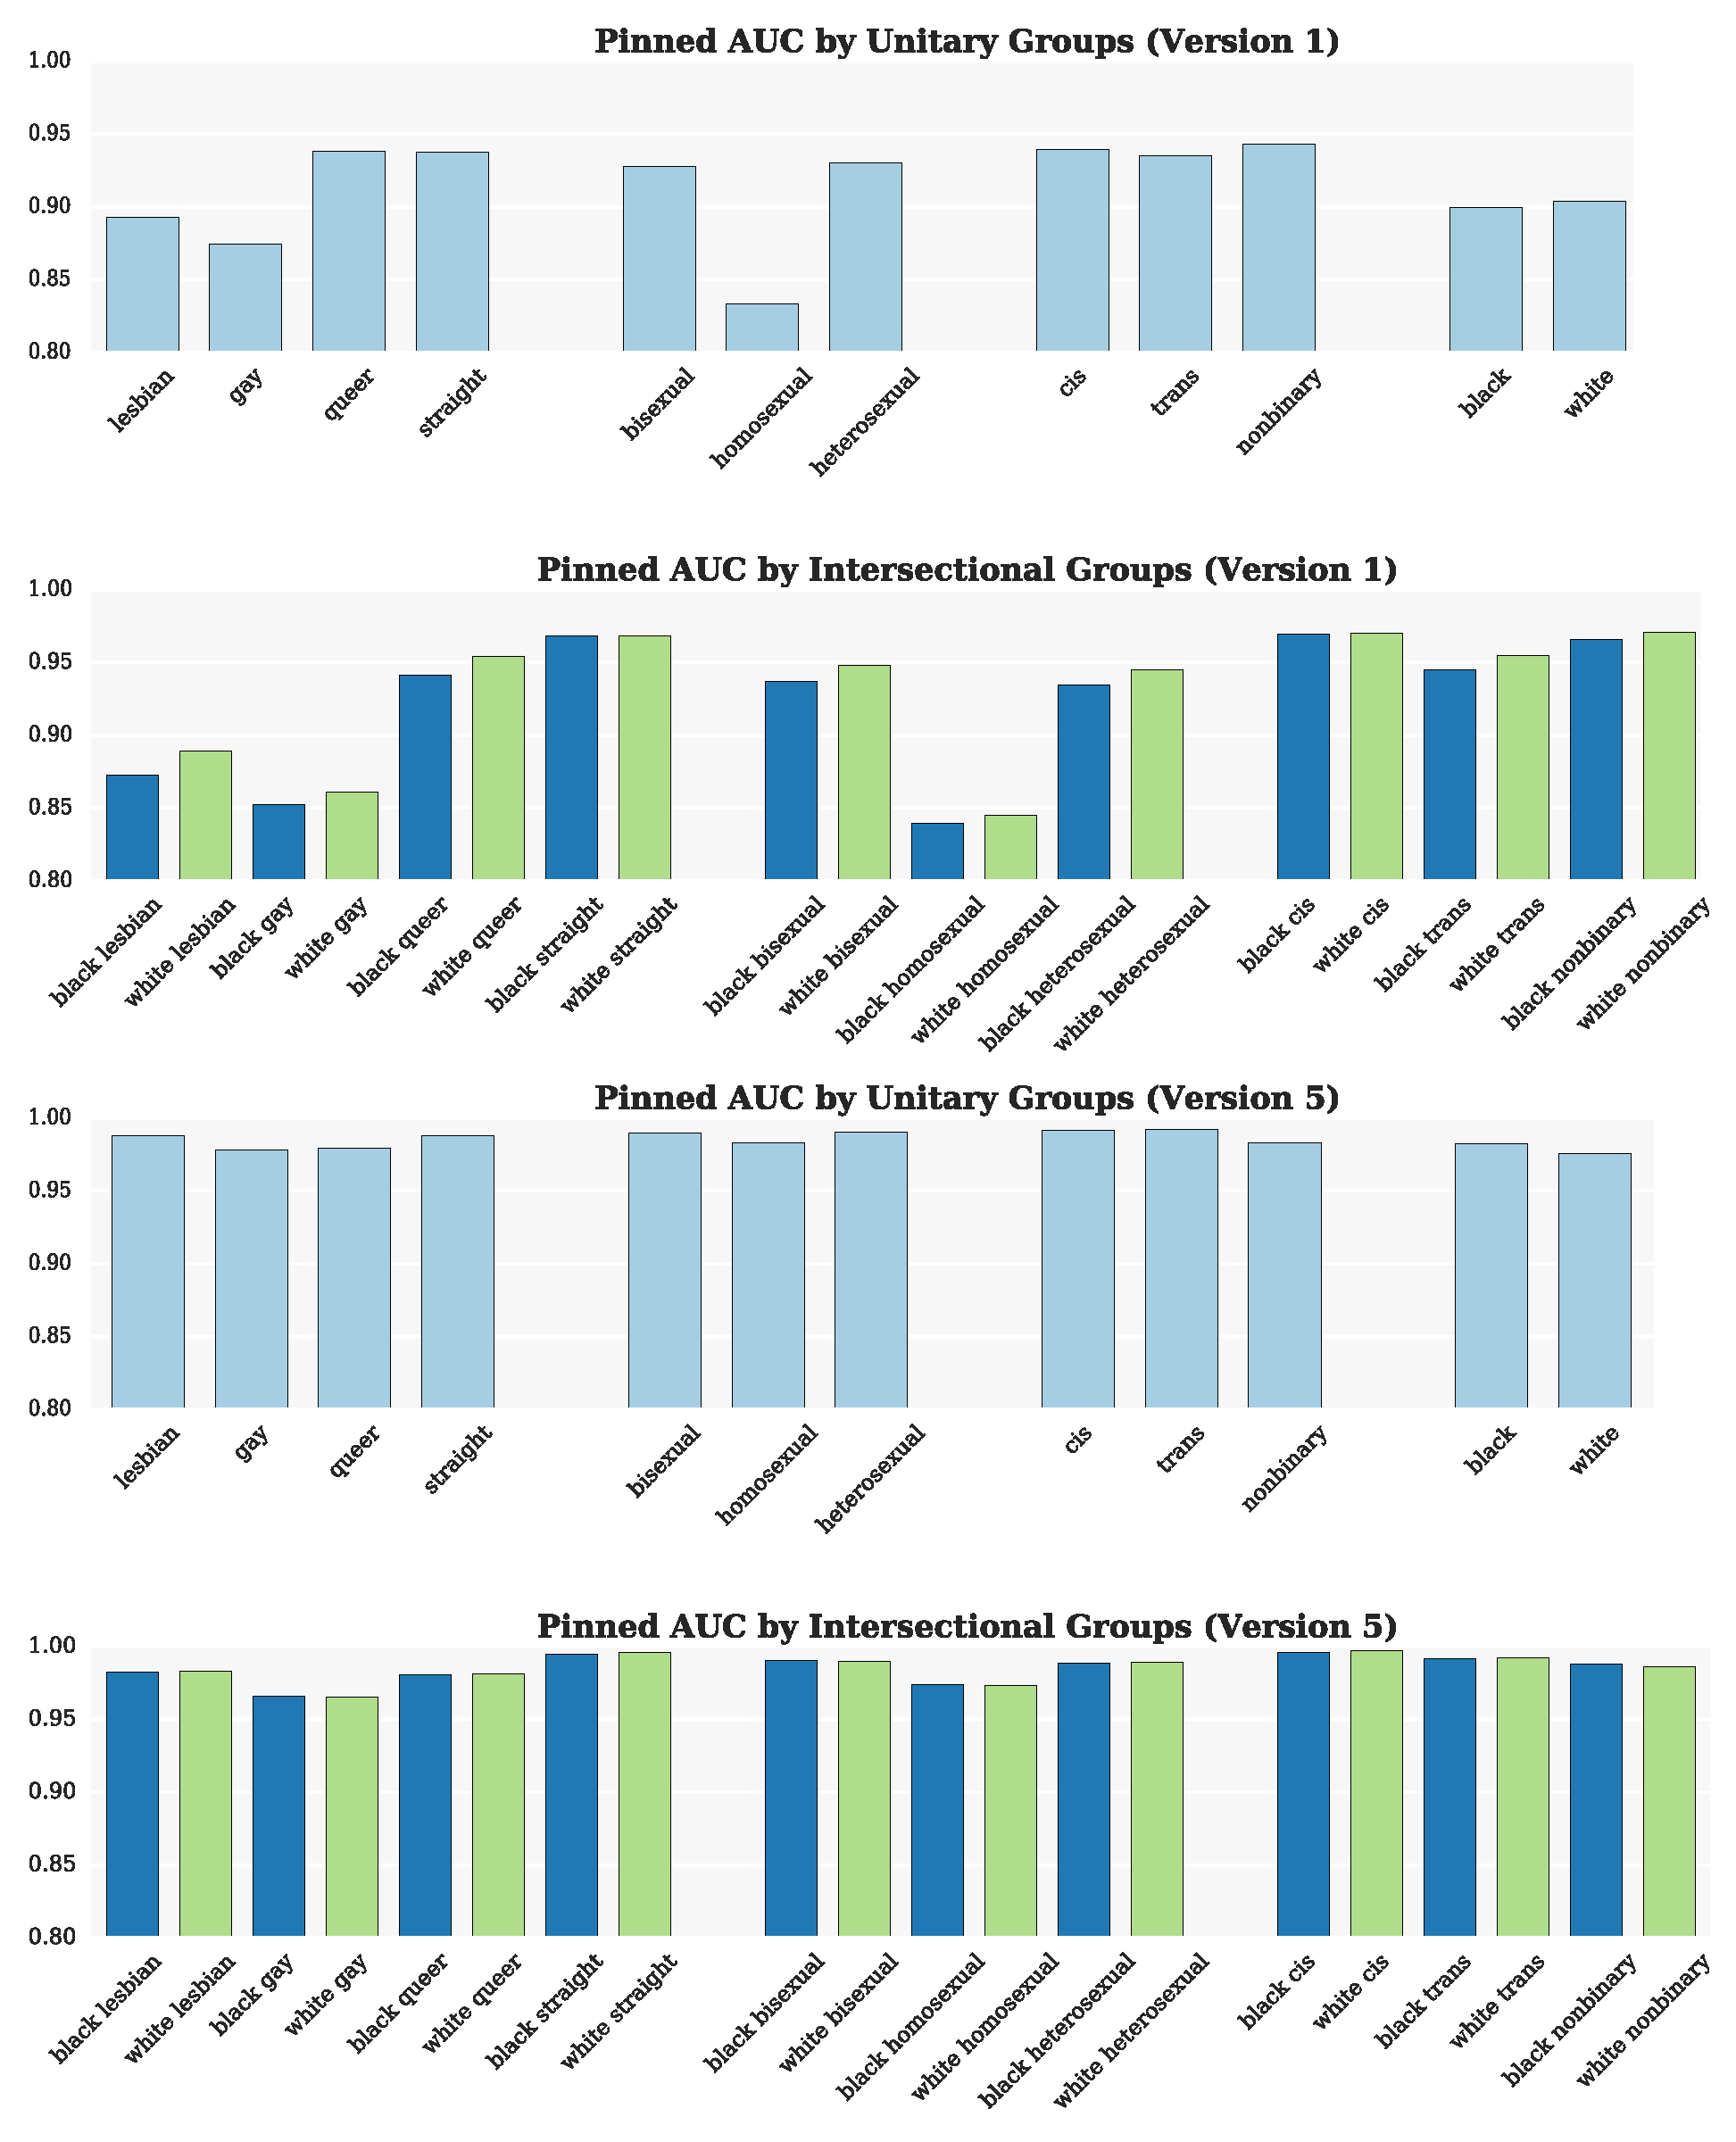
\includegraphics[scale=0.40]{pinned_auc_toxicity.pdf}
%{\bf Toxicity in Text (Version 1)
%}
\begin{tabular}{c@{}c}
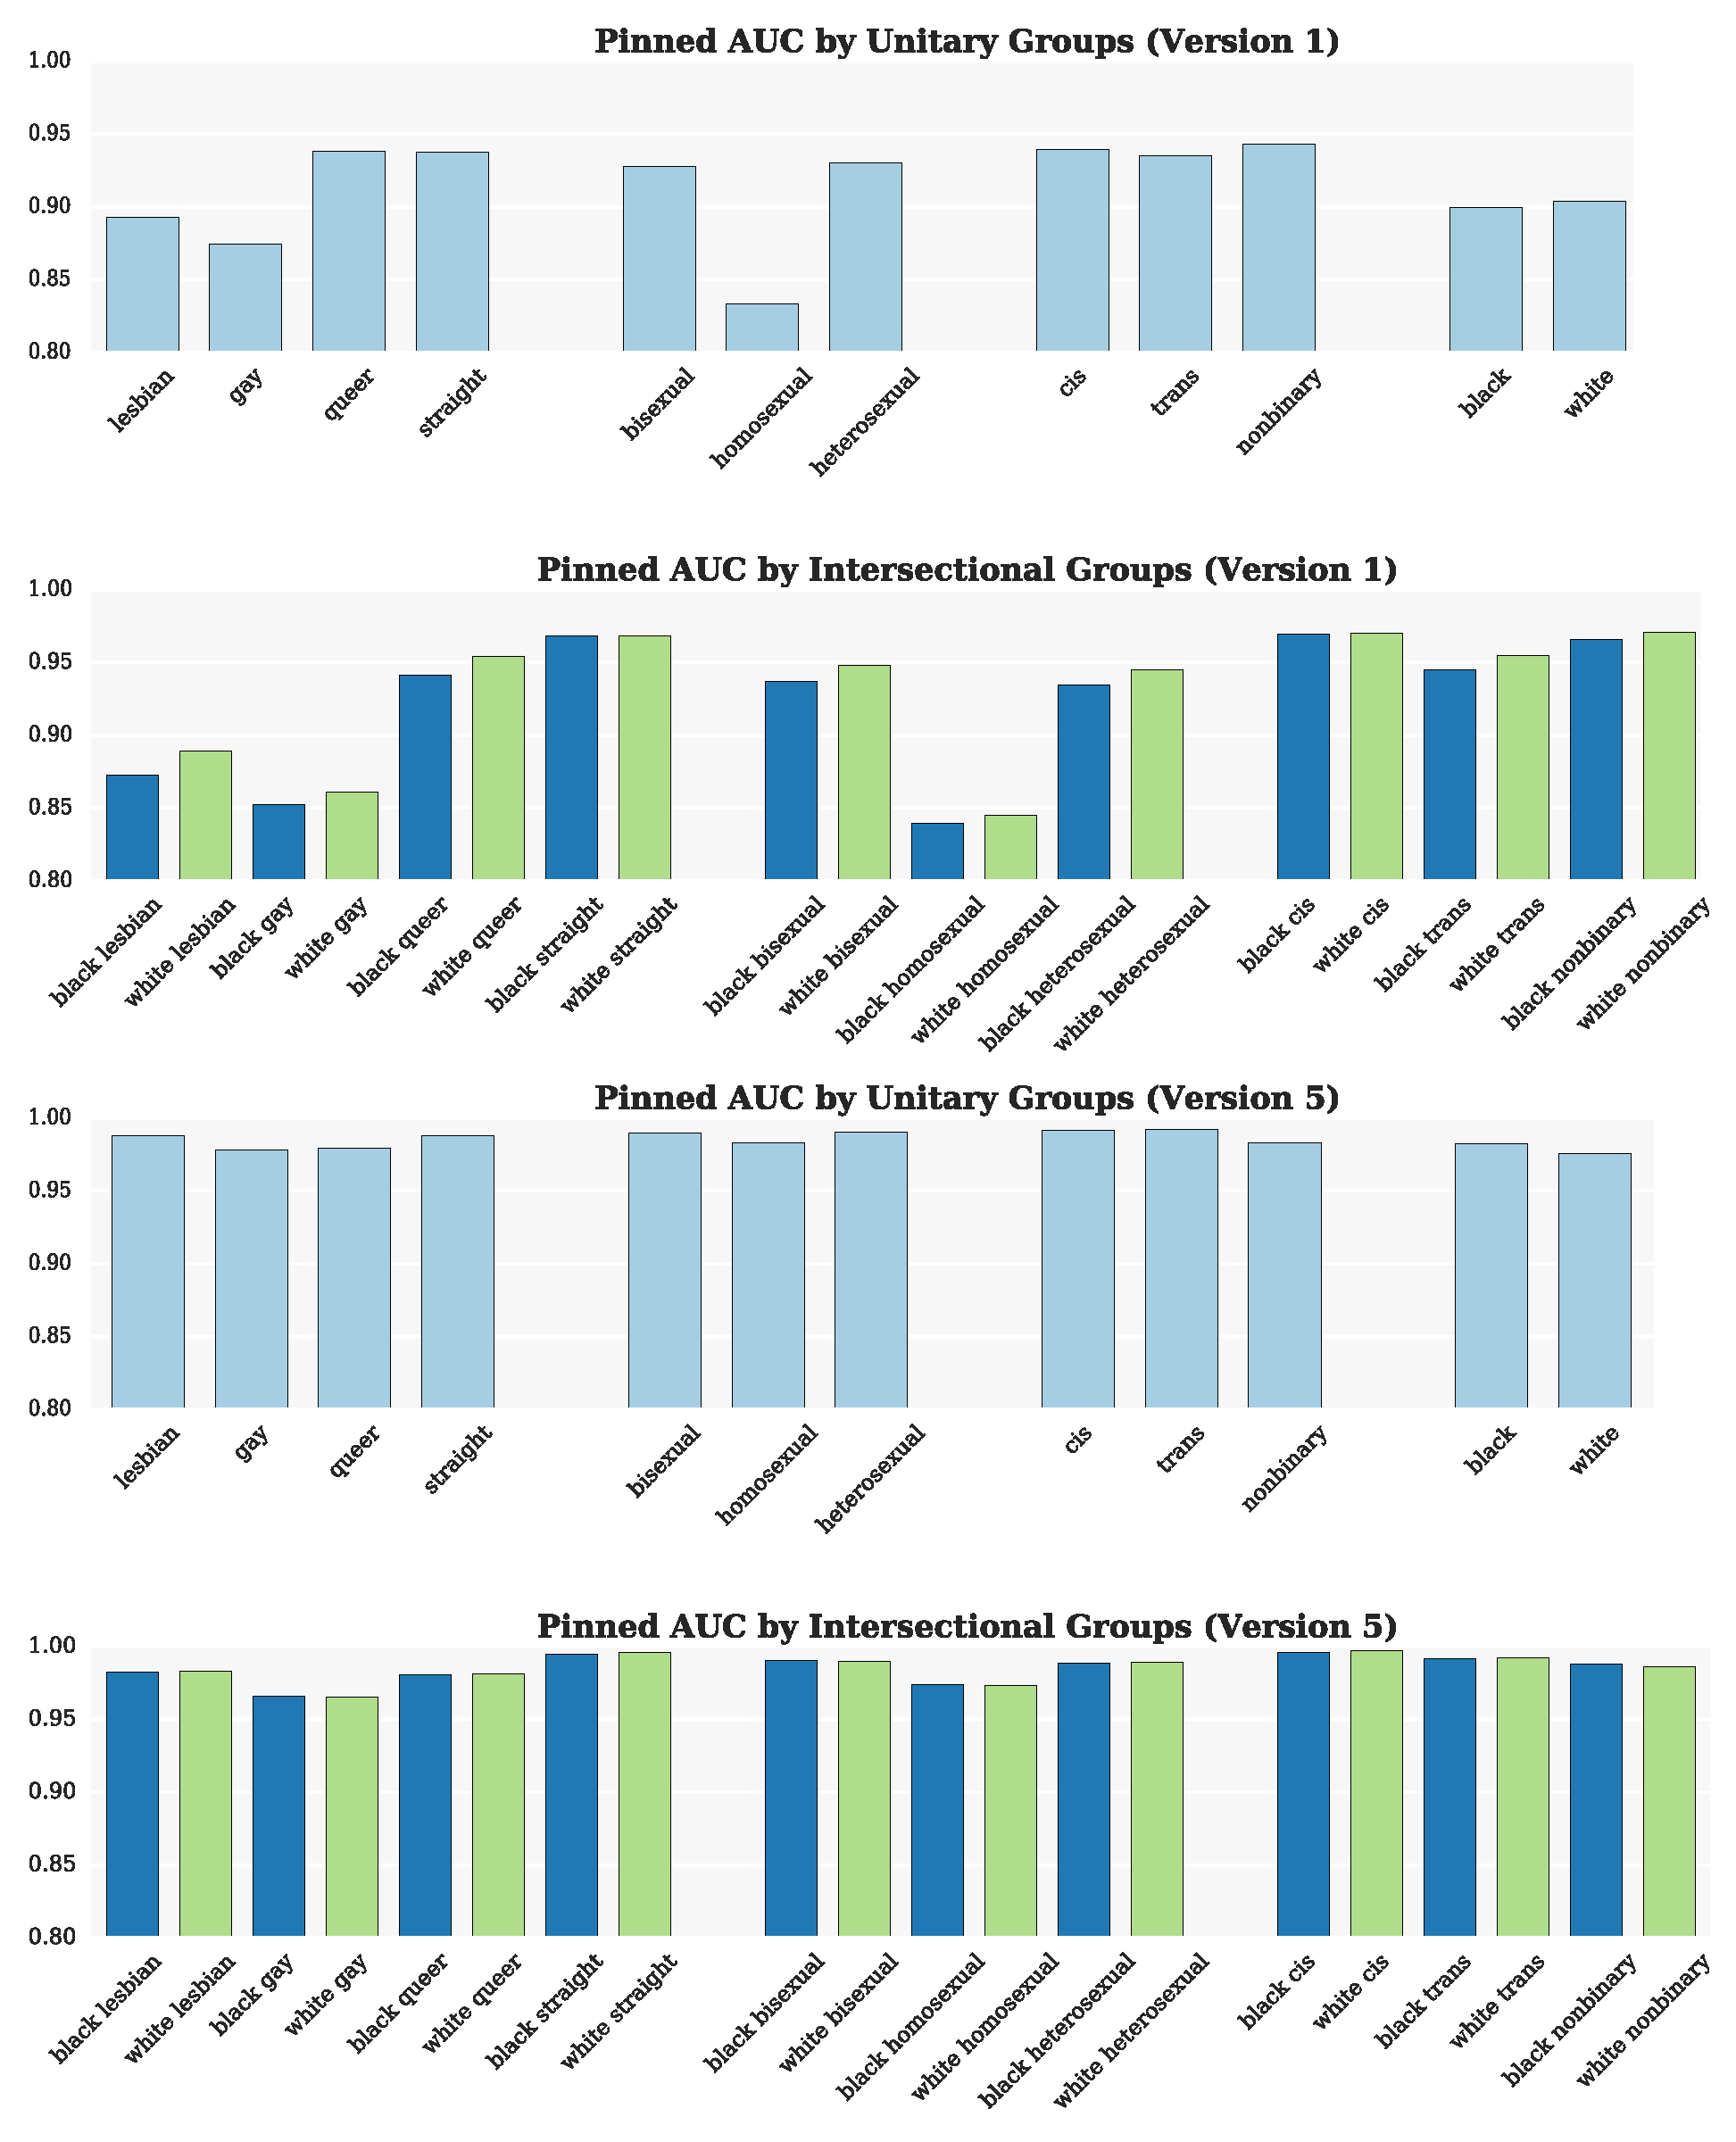
\includegraphics[scale=0.26,trim={0 20.1cm 0 0},clip]{pinned_auc_toxicity.pdf} & \vspace{.1em}\hspace{-.2em}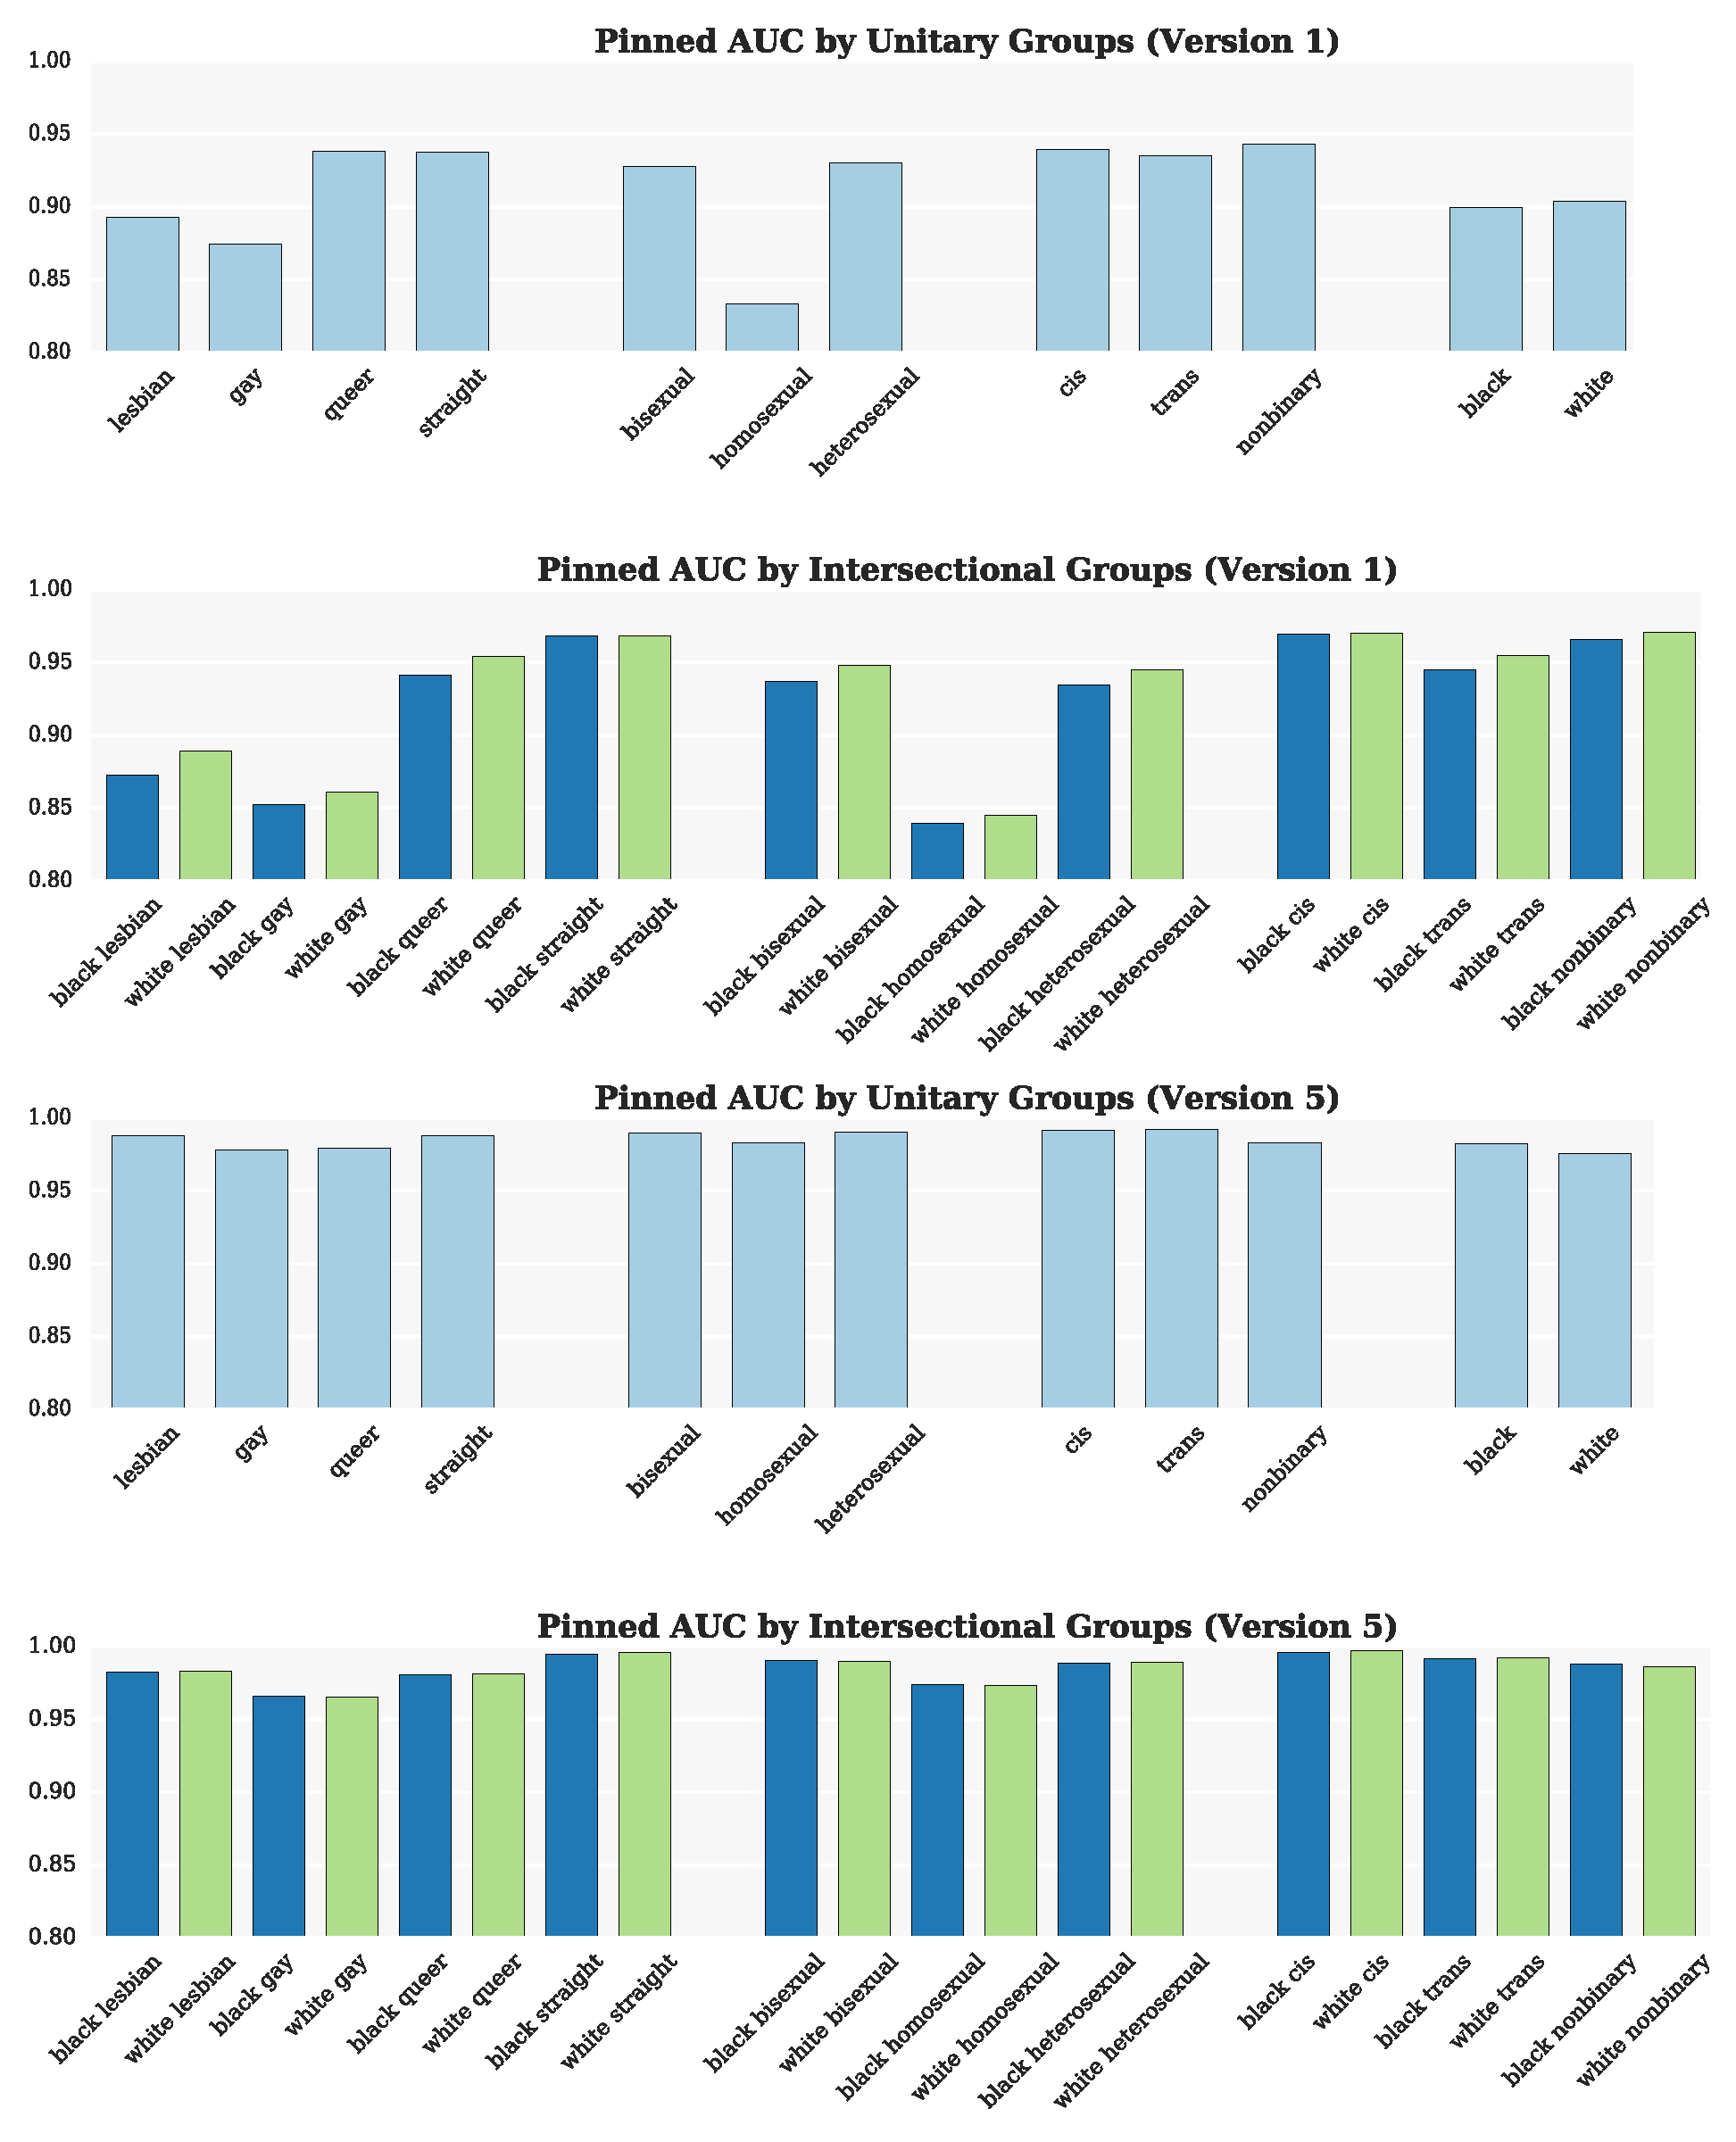
\includegraphics[scale=0.26,trim={0 0 0  20cm},clip]{pinned_auc_toxicity.pdf}
\end{tabular}

\end{subfigure}

%\end{framed}

%\begin{framed}
%{\bf Toxicity in Text (Version 5)
%}
%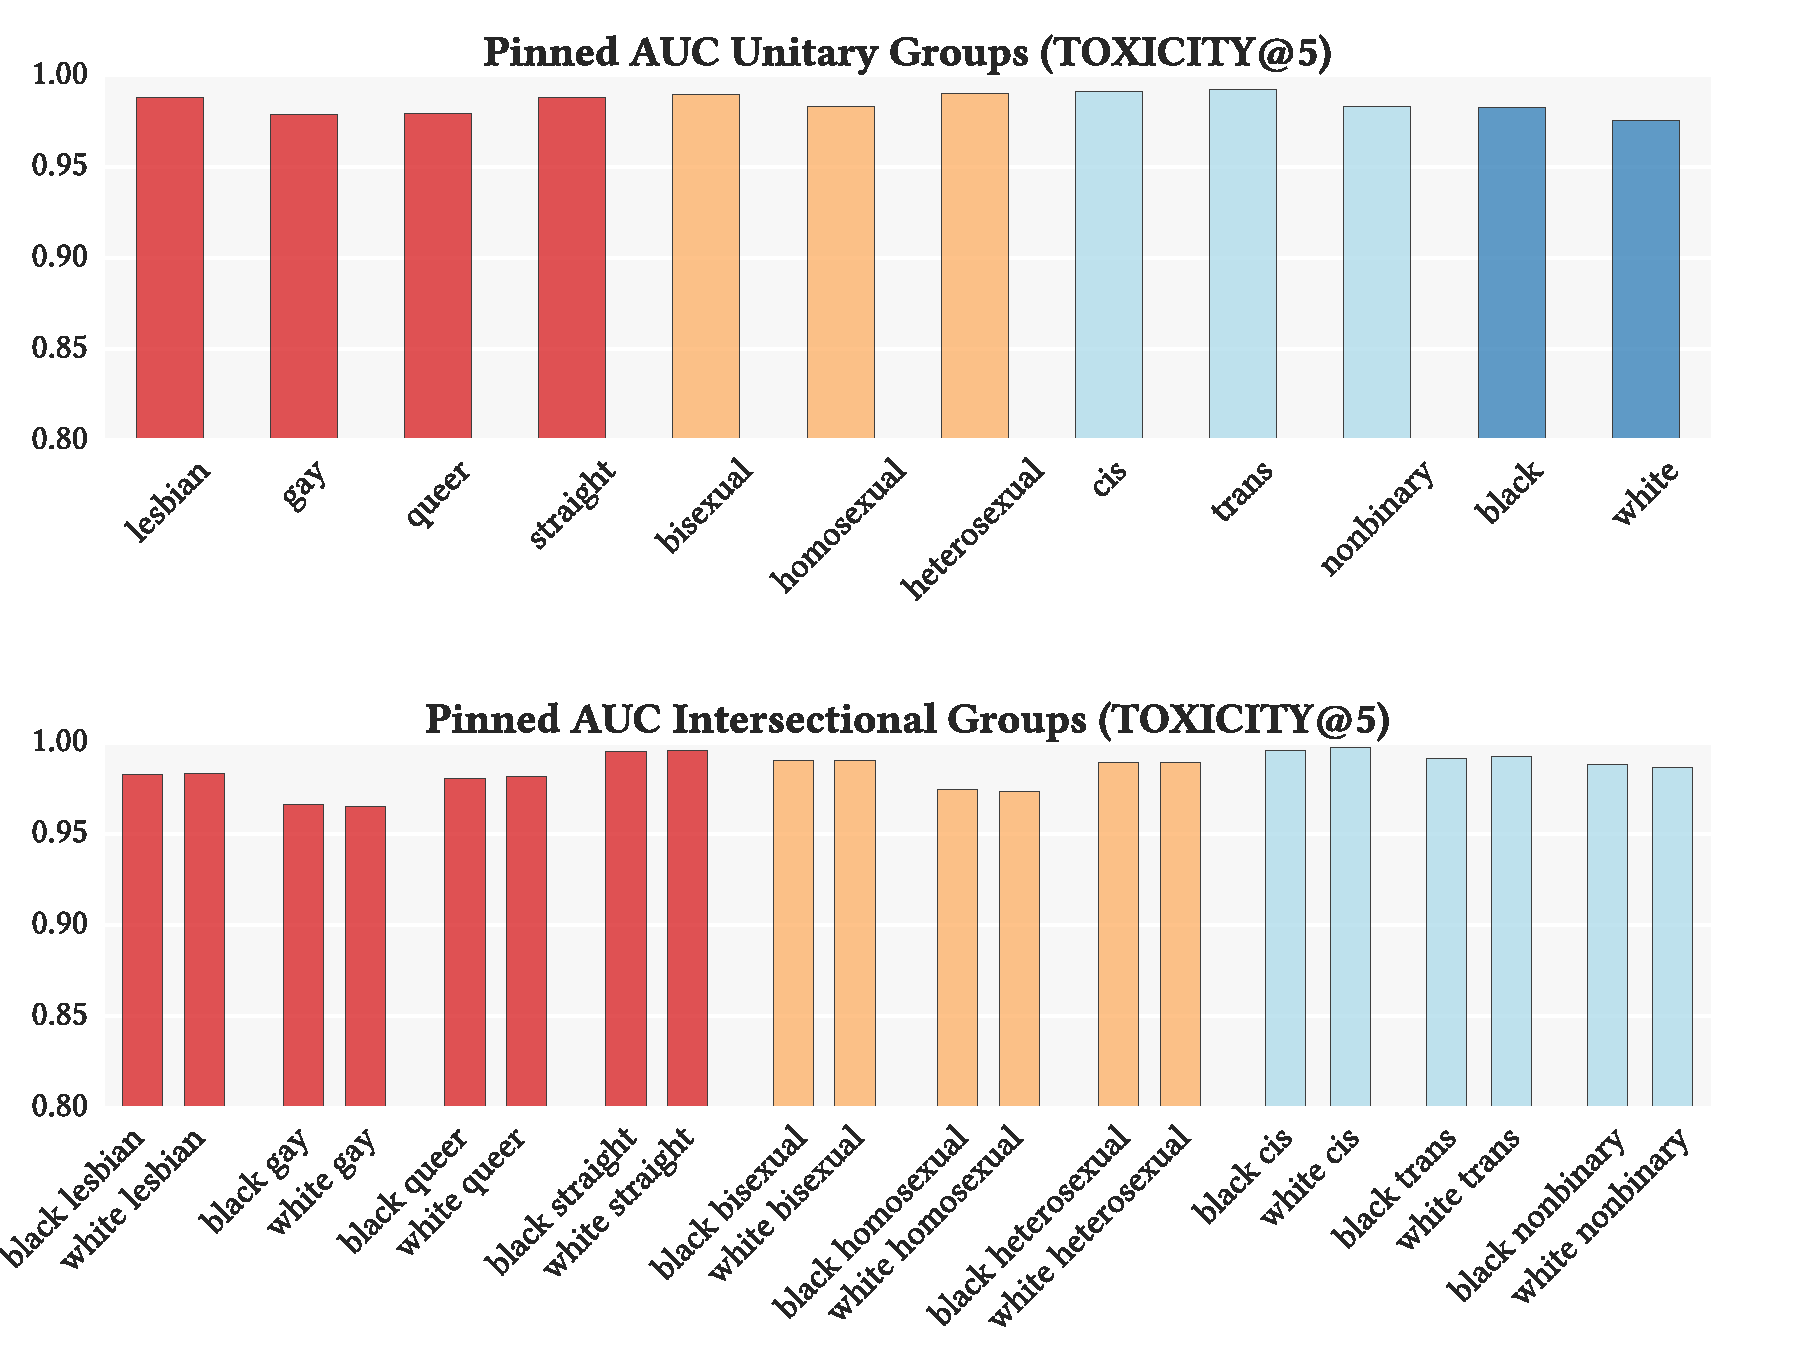
\includegraphics[scale=0.27]{toxicity_pinned_auc_5.pdf}
\end{framed}
\caption{Example Model Card for two versions of Perspective API's toxicity detector.}\label{fig:toxicity_card}\label{fig:toxicity_analysis}
\end{figure*}